\documentclass[a4paper,12pt]{article}
\usepackage{amsmath}
\usepackage{textcomp}
\usepackage{fancyhdr}
\usepackage{amssymb}
%\usepackage{psfig}
%\usepackage{amsmath}
%\usepackage[spanish]{babel} 
\usepackage{graphics}                 % Packages to allow inclusion of graphics
\RequirePackage{graphicx}
\usepackage{wrapfig}
\usepackage{caption}
\usepackage{comment}

\pagestyle{fancyplain} 
\long\def\symbolfootnote[#1]#2{\begingroup%
\def\thefootnote{\fnsymbol{footnote}}\footnote[#1]{#2}\endgroup} 

\hyphenation{ co-rres-pon-dien-tes cons-ta tem-pe-ra-tu-ra
              i-rre-ver-si-ble su-mi-nis-trar re-a-li-zan-do
              re-pre-sen-tar ne-ce-sa-rios pen-dien-tes
              res-pec-to di-fe-ren-tes de-sa-rro-lla-do
              io-ni-za-cion ra-san-tes co-li-sio-na-les
              de-ta-lla-re-mos par-ti-cu-lar es-cri-tu-ra
              De-sa-rro-lla-re-mos nues-tro nues-tros o-pe-ra-do-res
              de-ge-ne-ra-cio-nes de-ge-ne-ran a-su-mien-do 
              su-per-fi-cie co-rres-pon-dien-te po-si-ti-va vo-lu-men
              des-pla-za li-neal-men-te cons-tan-te o-rien-ta-do 
              des-pla-za-mien-to co-rrien-te}


\let\svthefootnote\thefootnote



\begin{document}

\lhead[\fancyplain{}]{Electromagnetismo}
\rhead[\fancyplain{}]{F5}

\begin{center}
{\Large \bf F\'{\i}sica 5$^{\mathrm{to}}$} \\
{\large \bf   Electromagnetismo}
\end{center}

%%%%%%%%%%%%%%%%%%%%%%%%%%%%%%%%%%%%%%%%%%%%%%%%%%%%%%%%%%%%%%%%%%%%%%%%
\vspace{0.05\textheight}
%%%%%%%%%%%%%%%%%%%%%%%%%%%%%%%%%%%%%%%%%%%%%%%%%%%%%%%%%%%%%%%%%%%%%%%%
\begin{enumerate}

\begin{minipage}{.6\textwidth}
\item 
\label{probespira}
Una barra conductora (Figura~\ref{fig:espira}), 
de largo $l=0.5$ m, es movida hacia la 
derecha, a una velocidad constante $\vec{v}$.
La barra se desplaza sobre dos rieles conductores, 
unidos en un extremo por una resistencia $R=2.00 ~\Omega$.
Durante todo el trayecto, atraviesa una regi\'on en la que 
existe un campo uniforme $\vec{B}=0.25$ T, saliente de la p\'agina. 
\begin{enumerate}
\item Calcular el valor de $v$, para que la corriente 
inducida sobre el circuito sea $I=5$ mA.
\item Indicar el sentido de esta corriente.
\item Calcular la potencia que disipa la resistencia.
\end{enumerate}
\end{minipage}
\begin{minipage}{.5\textwidth}
\begin{center}
 \hfill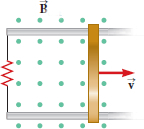
\includegraphics[width=0.9\textwidth,angle=0]
                        {figures/espira.jpg} 
\captionof{figure}{Prob.~\ref{probespira}.}
\label{fig:espira}
\end{center}
\end{minipage}

%%%%%%%%%%%%%%%%%%%%%%%%%%%%%%%%%%%%%%%%%%%%%%%%%%%%%%%%%%%%%%%%%%%%%%%%
\vspace{0.05\textheight}

\begin{minipage}{.6\textwidth}
\item 
\label{probespiras3}
Tres espiras se mueven cerca de un conductor muy largo, por el cual circula 
una corriente $I$, con las velocidades que se muestran  
la Figura~\ref{fig:espiras3}.
Dibujar las direcciones de las corrientes inducidas (si es que 
existen), en cada una de ellas.

\end{minipage}
\begin{minipage}{.5\textwidth}
\begin{center}
 \hfill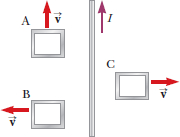
\includegraphics[width=0.9\textwidth,angle=0]
                        {figures/espiras3.jpg} 
\captionof{figure}{Prob.~\ref{probespiras3}}
\label{fig:espiras3}
\end{center}
\end{minipage}

%%%%%%%%%%%%%%%%%%%%%%%%%%%%%%%%%%%%%%%%%%%%%%%%%%%%%%%%%%%%%%%%%%%%%%%%

%%%%%%%%%%%%%%%%%%%%%%%%%%%%%%%%%%%%%%%%%%%%%%%%%%%%%%%%%%%%%%%%%%%%%%%%
\vspace{0.05\textheight}
\begin{minipage}{.6\textwidth}
\item 
\label{probcuadrado}
Dos espiras rectangulares se encuentran en el mismo plano, 
tal como lo indica la Figura~\ref{fig:cuadrado}. 
Sobre la espira externa circula una corriente $I$ con las 
siguientes caracter\'{\i}sticas:
\begin{enumerate}
\item Durante los 2 segundos iniciales, $I=250$ mA.
\item A partir de $t=2$ seg. comienza a disminuir linealmente, 
hasta anularse completamente, en $t=3$ seg.
\item A partir de $t=3$ seg. cambia su direcci\'on, llegando a 
$I=-250$ mA en un tiempo $t=4$ seg.
\item Entre este tiempo, y hasta $t=5$ seg., la corriente se mantiene 
en $I=-250$ mA.
\end{enumerate}
Indicar la direcci\'on de la corriente inducida en la 
espira interna (si es que existe), 
para $t=1,2.5,3,3.5$ y $4.5$ seg.

\end{minipage}
\begin{minipage}{.5\textwidth}
\begin{center}
 \hfill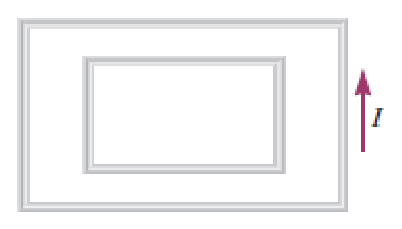
\includegraphics[width=0.9\textwidth,angle=0]
                        {figures/espirascuadradas.eps} 
\captionof{figure}{Prob.~\ref{probcuadrado}.}
\label{fig:cuadrado}
\end{center}
\end{minipage}

%%%%%%%%%%%%%%%%%%%%%%%%%%%%%%%%%%%%%%%%%%%%%%%%%%%%%%%%%%%%%%%%%%%%%%%%
\vspace{0.05\textheight}

\item Las especificaciones de un transformador para carga de tel\'efono 
celular enuncian: 
\begin{itemize}
\item Entrada: 220 V.
\item Salida: 5 V, 2 A.
\end{itemize}
Determine un n\'umero de espiras en el primario y en el secundario, 
con los cuales se puedan cumplir estos requisitos. 
Con esas caracter\'{\i}sticas, calcular la m\'{\i}nima corriente 
que debe circular por el primario.

 
%%%%%%%%%%%%%%%%%%%%%%%%%%%%%%%%%%%%%%%%%%%%%%%%%%%%%%%%%%%%%%%%%%%%%%%%

%%%%%%%%%%%%%%%%%%%%%%%%%%%%%%%%%%%%%%%%%%%%%%%%%%%%%%%%%%%%%%%%%%%%%%%%
\end{enumerate}
%%%%%%%%%%%%%%%%%%%%%%%%%%%%%%%%%%%%%%%%%%%%%%%%%%%%%%%%%%%%%%%%%%%%%%%%

%%%%%%%%%%%%%%%%%%%%%%%%%%%%%%%%%%%%%%%%%%%%%%%%%%%%%%%%%%%%%%%%%%%%%%%%
%%%%%%%%%%%%%%%%%%%%%%%%%%%%%%%%%%%%%%%%%%%%%%%%%%%%%%%%%%%%%%%%%%%%%%%%
\end{document}
